\RequirePackage[minted_workaround,caption_workaround,boxarc]{algo-common}
\ExplSyntaxOn
% Solution environment check (enable if SOLUTION=1)
\sys_get_shell:nnN { kpsewhich ~ --var-value ~ SOLUTION } { } \l_solution_env_var_tl
\tl_trim_spaces:N \l_solution_env_var_tl
\tl_if_eq:NnT \l_solution_env_var_tl {1} {\PassOptionsToClass{solution=true}{tudaexercise}}
\ExplSyntaxOff
\documentclass[accentcolor=3c,colorbacktitle,12pt]{tudaexercise}
% \usepackage[T1]{fontenc}
%\usepackage[utf8]{inputenc}
\ifPDFTeX
    \RequirePackage[utf8]{inputenc}
\fi
%\usepackage[ngerman]{babel}
%Includes
\usepackage[ngerman]{babel} %Deutsche Silbentrennung
\usepackage[utf8]{inputenc} %Deutsche Umlaute
\usepackage{float}
\usepackage{graphicx}
\usepackage{minted}
\RequirePackage{csquotes}
\RequirePackage{fontawesome5}

\DeclareGraphicsExtensions{.pdf,.png,.jpg}

\makeatletter
\author{Vorkursteam der Fachschaft Informatik}
\let\Author\@author

% dark mode
\ExplSyntaxOn
\IfDarkModeT{
    \cs_if_exist:NT \setbeamercolor {
        \setbeamercolor*{smallrule}{bg=.}
        \setbeamercolor*{normal~text}{bg=\thepagecolor,fg=.}
        \setbeamercolor*{background~canvas}{parent=normal~text}
        \setbeamercolor*{section~in~toc}{parent=normal~text}
        \setbeamercolor*{subsection~in~toc}{parent=normal~text,fg=.}
        \setbeamercolor*{footline}{parent=normal~text}
        \setbeamercolor{block~title~alerted}{fg=white,bg=white!20!\thepagecolor}
        \setbeamercolor*{block~body}{bg=black!70!gray!98!blue}
        \setbeamercolor*{block~body~alerted}{bg=\thepagecolor}
    }
    \cs_if_exist:NT \setbeamertemplate {
        \setbeamertemplate{subsection~in~toc~shaded}[default][50]
    }
}
\ExplSyntaxOff

% macros
\renewcommand{\arraystretch}{1.2} % Höhe einer Tabellenspalte minimal erhöhen
\newcommand{\N}{{\mathbb N}}
\renewcommand{\code}{\inputminted[]{python}}

\IfDarkModeTF{
    \newmintedfile[pythonfile]{python}{
        fontsize=\small,
        style=native,
        linenos=true,
        numberblanklines=true,
        tabsize=4,
        obeytabs=false,
        breaklines=true,
        autogobble=true,
        encoding="utf8",
        showspaces=false,
        xleftmargin=20pt,
        frame=single,
        framesep=5pt,
    }
    \newmintinline{python}{
        style=native,
        encoding="utf8"
    }
    \newmintinline{kotlin}{
        style=native,
        encoding="utf8"
    }


    \definecolor{codegray}{HTML}{eaf1ff}
    \newminted[bashcode]{awk}{
        escapeinside=||,
        fontsize=\small,
        style=native,
        linenos=true,
        numberblanklines=true,
        tabsize=4,
        obeytabs=false,
        breaklines=true,
        autogobble=true,
        encoding="utf8",
        showspaces=false,
        xleftmargin=20pt,
        frame=single,
        framesep=5pt
    }
}{
    \newmintedfile[pythonfile]{python}{
        fontsize=\small,
        style=friendly,
        linenos=true,
        numberblanklines=true,
        tabsize=4,
        obeytabs=false,
        breaklines=true,
        autogobble=true,
        encoding="utf8",
        showspaces=false,
        xleftmargin=20pt,
        frame=single,
        framesep=5pt,
    }
    \newmintinline{python}{
        style=friendly,
        encoding="utf8"
    }
    \newmintinline{kotlin}{
        style=friendly,
        encoding="utf8"
    }

    \definecolor{codegray}{HTML}{eaf1ff}
    \newminted[bashcode]{awk}{
        escapeinside=||,
        fontsize=\small,
        style=friendly,
        linenos=true,
        numberblanklines=true,
        tabsize=4,
        obeytabs=false,
        breaklines=true,
        autogobble=true,
        encoding="utf8",
        showspaces=false,
        xleftmargin=20pt,
        frame=single,
        framesep=5pt
    }
}

\let\origpythonfile\pythonfile
\renewcommand{\pythonfile}[1]{\pythonfileh{#1}{}}
\newcommand{\pythonfileh}[2]{\origpythonfile[#2]{#1}}

\DeclareDocumentCommand{\kotlinfile}{O{} O{} m}{\inputCode[#1]{minted language=kotlin,#2}{#3}}

\newcommand*{\ditto}{\texttt{\char`\"}}

\newcommand{\shellprefix}{\textcolor{TUDa-3a}{\ttfamily\bfseries \$~}}
\DeclareTCBListing{commandshell}{ O{} O{} }{
    colback=\IfDarkModeTF{black}{black!80},
    colupper=white,
    colframe=TUDa-3a,
    listing only,
    % listing options={style=tcblatex,language=sh},
    listing engine=minted,
    minted style=dracula,
    minted options={
        % linenos=true,
        numbersep=3mm,
        texcl=true,
        autogobble,
        escapeinside=@@,
        breaklines,
        highlightcolor=yellow!50!black,
        #1
    },
    #2,
    % before upper={\textcolor{red}{\small\ttfamily\bfseries root \$> }},
    % every listing line={\textcolor{red}{\small\ttfamily\bfseries root \$> }}
}

\usepackage{hyperref}
\usepackage{ifthen}
\usepackage{listings}
%\usepackage{graphicx}
\usepackage{multicol}
\usepackage{multirow}
\usepackage{amssymb}
\RequirePackage{silence}
\WarningFilter[sillyfonterror]{latex}{Font~shape~declaration~has}
\ActivateWarningFilters[sillyfonterror]
\ifLuaTeX
    % Fix Font warnings for mathdesign
    \DeclareFontFamily{TU}{mdbch}{}
    \DeclareFontShape{TU}{mdbch}{m}{n}{
        <-> \UnicodeFontFile{lmroman10-regular}{\UnicodeFontTeXLigatures}
    }{}
    \RequirePackage[utf8]{luainputenc} % if problems with ß exist
\fi

\definecolor{darkblue}{rgb}{0,0,.5}
\hypersetup{colorlinks=true, breaklinks=true, linkcolor=\IfDarkModeTF{cyan}{darkblue}, menucolor=darkblue, urlcolor=\IfDarkModeTF{cyan}{darkblue}}

% configuration
\makeatletter
\@ifundefined{c@ex}{
    \newcounter{ex}\setcounter{ex}{1}
}{}
\makeatother
\IfDarkModeT{
    \selectcolormodel{RGB}
}
\newboolean{sln}\setboolean{sln}{false}
\newboolean{SoSe}\setboolean{SoSe}{false}
\newcommand{\thenextyear}{\the\numexpr\year+1\relax}
%

\newcommand{\ext}{py}
\newcommand{\sln}[1]{\ifthenelse{\boolean{sln}}{\subsubsection*{Antwort}{\itshape #1}}{}}
\newcommand{\slnformat}[1]{\ifthenelse{\boolean{sln}}{#1}{}}
\newcommand{\vorkurstaskformat}[1]{\ifthenelse{\boolean{sln}}{}{#1}}
\newcommand{\vorkurstask}[1]{\input{task/#1}\IfFileExists{./sln/#1.tex}{\sln{\input{sln/#1}}}{\IfFileExists{./sln/#1.\ext}{\sln{\pythonfile{sln/#1.\ext}}}{\ClassError{Vorkurs-TeX}{No solution specified for task #1}{Add solution file #1.tex or #1.\ext}}}}
\newcommand{\mccmd}{Kreuze zu jeder Antwort an, ob sie zutrifft (\textbf{w}) oder nicht (\textbf{f}).}
\newcommand{\mchead}{\item[\textbf{w} \textbf{f} ]}
\newcommand{\mcitem}[1]{\item[$\square\ \square$] #1}
\newcommand{\mcitemt}[1]{\item[$\ifthenelse{\boolean{sln}}{\blacksquare}{\square}\ \square$] #1}
\newcommand{\mcitemf}[1]{\item[$\square\ \ifthenelse{\boolean{sln}}{\blacksquare}{\square}$] #1}
\newcommand{\ptitle}{\ifthenelse{\boolean{SoSe}}{Sommersemester \the\year}{Wintersemester \the\year/\thenextyear}}

\newcommand{\lstinlinenoit}[1]{\upshape{\lstinline|#1|}\itshape}
\lstset{language=Python, basicstyle=\ttfamily\small, keywordstyle=\color{\IfDarkModeTF{cyan!60!black}{blue!80!black}}, identifierstyle=, commentstyle=\color{green!50!.}, stringstyle=\ttfamily,
    tabsize=4, breaklines=true, numbers=left, numberstyle=\small, frame=single, backgroundcolor=\color{blue!3!\thepagecolor}}
\author{Fachschaft Informatik}

\newcommand{\stage}[1]{(\ifcase#1\or{Einstieg}\or{Vertiefung}\or{Herausforderung}\else\fi)}
\newcommand{\bonus}[1]{\textit{BonusFact: }#1}

\sheetnumber{1}
\title{Aufgaben Programmiervorkurs}
\subtitle{von der Fachschaft Informatik\hfill\ptitle}

\usepackage{hyperref}
\usepackage{wrapfig}

\begin{document}
\maketitle{}

\begin{task}[points=auto]{Einleitung}
    \begin{subtask*}[points=0]{Kotlin Installieren}
        Hey, willkommen bei den Übungen zum Programmiervorkurs im \ptitle. Wie in der
        Vorlesung verwenden wir für die Übungen die Programmiersprache Kotlin. \\\\
        %
        Für das Installieren und Starten von Kotlin haben wir eigene Guides in Moodle verlinkt.
        Folgt denen, sodass ihr Kotlin ausführen könnt.
        \begin{solution}
            Kotlin ist installiert und dem Pfad hinzugefügt. Der Befehl
            \mintinline{text}{kotlin -version} gibt eine Versionsnummer von mindestens \mintinline{text}{1.8.22} aus.
            % Der Kotlin Interpreter mit \mintinline{text}{kotlin} wurde gestartet.

            Das Repl wurde korrekt installiert und mit \mintinline{text}{ki} gestartet. Der Befehl
            \mintinline{text}{ki} gibt eine Versionsnummer von mindestens \mintinline{text}{0.5.2} aus.
        \end{solution}
    \end{subtask*}
    \begin{subtask*}[points=0]{Theoriefragen}
        \subsection{Theoriefragen}
        \begin{itemize}
            \mchead
            \mcitemt{Programmcode steht üblicherweise in Textdateien}
            \mcitemf{Ein Prozessor kann Kotlin direkt ausführen}
            \mcitemt{Um Kotlin-Code auszuführen kann ein Compiler verwendet werden}
            \mcitemf{Es ist niemals sinnvoll seinen Code mit Kommentaren zu überladen}
        \end{itemize}
        \begin{solution}
            Die zutreffenden Antworten sind die Aussagen 1 und 3.
        \end{solution}
    \end{subtask*}
\end{task}
\begin{task}[points=auto]{Ausdrücke \stage1}
    \begin{subtask*}[points=0]{Frage \& Antwort}
        Gebt nacheinander die folgenden Ausdrücke in \kotlininline{ki} ein. Drückt nach
        jedem Eintrag \textit{ENTER}, um den Ausdruck auszuwerten. Was passiert?
        Versucht, zu erklären, warum. Probiert auch noch weitere Ausdrücke, die euch
        einfallen.

        \begin{multicols}{3}
            \begin{itemize}
                \item \mintinline{text}{2}
                \item \mintinline{text}{10.0}
                \item \mintinline{text}{"1"}
                \item \mintinline{text}{'1'}
                \item \mintinline{text}{Test}
                \item \mintinline{text}{"Test"}
                \item \mintinline{text}{0x11}
                \item \mintinline{text}{0b11}
                \item \mintinline{text}{true}
                \item \mintinline{text}{True}
                \item \mintinline{text}{false}
                \item \mintinline{text}{False}
            \end{itemize}
        \end{multicols}

        \bonus{Kotlin gibt nicht nur den Wert eines Ausdrucks,
            sondern auch seinen Typ an.}

        \begin{solution}
            Zahlen ohne Anführungszeichen ergeben die Zahl. Rationale Zahlen brauchen einen
            Dezimal\fatsf{punkt}. Doppelte Anführungszeichen (\mintinline{text}{"}) ergeben Strings,
            der Prefix \mintinline{text}{0x} erwartet hexadezimales Format, der Prefix \mintinline{text}{0b}
            binäres Format. Wahrheitswerte müssen klein geschrieben werden (\kotlininline{true},
            \kotlininline{false}).
            Einfache Anführungszeichen ergeben Chars, hier wird ein einzelnes Zeichen als numerischer Wert abgespeichert.
            Strings sind dann die Verkettung von Chars.
        \end{solution}
    \end{subtask*}
    \begin{subtask*}[points=0]{Mathe 0 für Informatiker*innen}
        Wenn euch das Programm aber nur das zurückgeben könnte, was ihr hinschreibt,
        dann wäre das ja noch lange kein \textit{Computer}. Darum rechnen wir nun etwas.
        Überlegt euch was die folgenden Ausdrücke ergeben, und was die verwendeten
        Symbole für Operationen bezeichnen. Beachtet dabei, die Operatorenpräzedenz.

        \begin{multicols}{3}
            \begin{itemize}
                \item \kotlininline{16 + 26}
                \item \kotlininline{13.75 + 28.67}
                \item \kotlininline{2 * 3 + 6 * 6}
                \item \kotlininline{"4" + 2}
                \item \kotlininline{12 * 133 / 28 - 15}
                \item \kotlininline{'a' + 5}
                \item \kotlininline{1.3 * 5.6}
            \end{itemize}
        \end{multicols}

        \bonus{Weitere mathematische Operationen können mit \kotlininline{import kotlin.math.*} importiert werden.

            \begin{multicols}{3}
                \begin{itemize}
                    \item \kotlininline{PI}
                    \item \kotlininline{12.0.pow(3)}
                    \item \kotlininline{sqrt(2.0)}
                \end{itemize}
            \end{multicols}}

        \begin{solution}
            Das Ergebnis ist meistens eine Variante von \kotlininline{42}.
            Wichtig ist, dass hier Punkt- vor Strichrechnung gilt.
            Beachtet die unterschiedlichen Datentypen.
            Die letzte Aufgabe betont, dass manche Operationen auf Kommazahlen keine genauen Ergebnisse liefern.
        \end{solution}
    \end{subtask*}
\end{task}
\begin{task}[points=auto]{Konvertierung \stage2}
    \begin{subtask*}[points=0]{Konvertierung}
        Nehmen wir mal an, ihr habt den Text \kotlininline{"1000"} zur Verfügung. Vielleicht
        errechnet; vielleicht aus einer API (\textit{application programming interface}, allgemeine Bezeichnung für Schnittstellen zwischen Programmen)? Es kommt immer wieder vor, dass die Daten noch den falschen Typ haben, wenn ihr sie bekommt.

        Gebt die folgenden Ausdrücke ein, und findet das Ergebnis heraus.

        \textit{Hinweis: es kann sein, dass einige Konvertierungen fehlschlagen. In diesem Fall überlegt euch, warum. Die Fehlermeldung kann dabei hilfreich sein.}

        \begin{multicols}{3}
            \begin{enumerate}
                \item \kotlininline{"100".toInt()}
                \item \kotlininline{"1.3".toDouble()}
                \item \kotlininline{"NaN".toDouble()}
                \item \kotlininline{123.toString()}
                \item \kotlininline{"0x11".toInt()}
                \item \kotlininline{2.toString() + "5"}
                \item \kotlininline{(2 + 5).toString()}
                \item \kotlininline{5.toDouble()}
                \item \kotlininline{5.5.toInt()}
                \item \kotlininline{"4.2".toInt()}
            \end{enumerate}
        \end{multicols}

        \begin{solution}
            \begin{multicols}{3}
                \begin{enumerate}
                    \item \kotlininline{kotlin.Int = 100}
                    \item \kotlininline{kotlin.Double = 1.3}
                    \item \kotlininline{kotlin.Double = NaN}
                    \item \kotlininline{kotlin.String = 123}
                    \item \kotlininline{NumberFormatException}
                    \item \kotlininline{kotlin.String = 25}
                    \item \kotlininline{kotlin.String = 7}
                    \item \kotlininline{kotlin.Double = 5.0}
                    \item \kotlininline{kotlin.Int = 5}
                    \item \kotlininline{NumberFormatException}
                \end{enumerate}
            \end{multicols}
        \end{solution}
    \end{subtask*}
    \begin{subtask*}[points=0]{Verrückte Eingabe \stage3}
        Versucht einen Ausdruck zu finden, der nur \kotlininline{'1'}, \kotlininline{0},
        \kotlininline{toInt}, \kotlininline{toString} und Operationen verwendet, der
        insgesamt zu \kotlininline{3000} auswertet. Beachtet, dass solche Ausdrücke
        wie ihr hier schreiben sollt, so \textbf{niemals} in echtem Code auftauchen
        sollten.

        \textit{Hinweis: Zwar soll am Ende eine Zahl rauskommen, ihr werdet aber in dieser Aufgabe oft zwischen Zahl und Text hin- und herkonvertieren müssen.}

        \begin{solution}
            \begin{codeBlock}[]{minted language=kotlin}
                >>> (("1".toInt() + "1".toInt() + "1".toInt()).toString() + 0.toString() + 0.toString() + 0.toString()).toInt()
                res4: kotlin.Int = 3000
            \end{codeBlock}
            Es gibt natürlich auch noch andere Möglichkeiten.
        \end{solution}
    \end{subtask*}
\end{task}
\begin{task}[points=auto]{Fehler}
    \begin{subtask*}[points=0]{Fehlertypen \stage1}

        Ordnet die folgenden drei Fehlertypen den folgenden Ausdrücken zu.
        \begin{multicols}{3}
            \begin{itemize}
                \item[] \textbf{expecting an expression}
                \item[] \textbf{ArithmeticException}
                \item[] \textbf{unresolved reference}
            \end{itemize}
            \begin{itemize}
                \item[] \kotlininline{True}
                \item[] \kotlininline{2.toInt)3(}
                \item[] \kotlininline{2 / 0}
            \end{itemize}
            \begin{itemize}
                \item[] \textit{Syntaktischer Fehler}
                \item[] \textit{Lexikalischer Fehler}
                \item[] \textit{Semantischer Fehler}
            \end{itemize}
        \end{multicols}

        \begin{solution}
            \begin{enumerate}
                \item \kotlininline{True} ist ein falsch geschriebenes Schlüsselwort und somit ein \\
                    lexikalischer Fehler (unresolved reference)
                \item \kotlininline{2.toInt)3(} hat die Klammern vertauscht, somit ein \\
                    syntaktischer Fehler (expecting an expression)
                \item \kotlininline{2 / 0} ist eine undefinierte Rechnung, also ein
                    \\ semantischer Fehler (\textbf{ArithmeticException})
            \end{enumerate}

        \end{solution}
    \end{subtask*}
    \begin{subtask*}[points=0]{Finde den Fehler \stage2}
        Gegeben sind die folgenden Listings. Führt die Programme aus und beschreibt, warum jeweils ein Fehler auftritt.
        \begin{codeBlock}[]{minted language=kotlin}
            >>> prinntln("Hello World") // a)
            >>> println(Hello World!)    // b)
            >>> println("Alter: " * 18)  // c)
            >>> println("Hello World!)   // d)
        \end{codeBlock}
        \begin{solution}
            \begin{enumerate}
                \item \mintinline{text}{unresolved reference: prinntln}: Ein \textcolor{red}{Lexikalischer Fehler}, da es keine Funktion mit dem angegebenen Namen
                    \mintinline{text}{prinntln} gibt. Gültig wäre \mintinline{text}{println}. Ein klassische Tippfehler.
                \item Ein \textcolor{red}{Syntaktischer Fehler}, da Strings immer in einfachen oder doppelten Anführungszeichen
                    stehen müssen.
                \item \mintinline{text}{Unresolved reference}: Ein \textcolor{red}{Semantischer Fehler}, da Texte und Zahlen multiplizierbar sind.
                    \textbf{Bonus Fact}: Hierfür kann man z.B. \kotlininline{"Hallo ".repeat(3)} nutzen.
                \item Ein \textcolor{red}{Syntaktischer Fehler}, da der Rest der Zeile nun auch als String gelesen wird, der aber nie endet.
            \end{enumerate}

        \end{solution}
    \end{subtask*}
\end{task}
\begin{task}[points=auto]{Challenge}
    \begin{subtask*}[points=0]{Caesar Cipher \stage3}
        \begin{wrapfigure}[7]{r}{0.2\textwidth}
            \begin{center}
                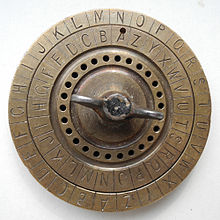
\includegraphics{caesar-cipher.jpg}
            \end{center}
            Quelle: Wikipedia
        \end{wrapfigure}
        Wir wollen einen sehr einfaches Verschlüsselungsverfahren implementieren, den Caesar Cipher\footnote{\url{https://de.wikipedia.org/wiki/Caesar-Verschlüsselung}}.
        Grundidee ist, das Alphabet auf zwei Scheiben zu schrieben und diese gegeneinander zu drehen.
        Eine Verschiebung von $5$ wäre zum Beispiel:
        \begin{align*}
            \text{\kotlininline{'A'}} \to \text{\kotlininline{'F'}} \\
            \text{\kotlininline{'B'}} \to \text{\kotlininline{'G'}} \\
            \text{\kotlininline{'M'}} \to \text{\kotlininline{'R'}}
        \end{align*}

        Geben sollen eine Verschiebung von \kotlininline{5} und ein beliebiger Char sein.
        Es soll einmal die Ver- und die Entschlüsselung berechnet werden.
        Man muss natürlich aufpassen, dass man bei z.B.
        \kotlininline{'A'} nicht \enquote{zu weit nach links} geht.

        \begin{solution}
            Ein Beispiel für die Verschlüsselung wäre die folgende Rechnung:
            \begin{codeBlock}[]{minted language=kotlin}
                'A' + ((@\textit{\color{accentcolor}<unverschlüsselter char>}@ - 'A') + 5) % 26
            \end{codeBlock}
            Und für die Entschlüsselung die folgende Rechnung:
            \begin{codeBlock}[]{minted language=kotlin}
                'A' + ((@\textit{\color{accentcolor}<verschlüsselter char>}@ - 'A') - 5 + 26) % 26
            \end{codeBlock}
            Dabei sollen \texttt{\textit{\color{accentcolor}<unverschlüsselter char>}} und \texttt{\textit{\color{accentcolor}<verschlüsselter char>}} jeweils mit entsprechenden Wert ersetzt werden.
            Z.B. würde \kotlininline{'B'} verschlüsselt zu \kotlininline{'G'} und das verschlüsselte \kotlininline{'G'} hier wieder zu \kotlininline{'B'}.

            Wobei man hier allerdings aufpassen muss, ist wenn der zu verschlüsselnde Buchstabe soweit hinten im Alphabet ist, dass man wieder zum Anfang springen muss. Wenn man z.B. \kotlininline{'X'} verschlüsseln will, dann soll das Ergebnis \kotlininline{'C'} sein. Wenn man das \kotlininline{'C'} dann wieder entschlüsseln will soll man wieder bei \kotlininline{'X'} raus kommen. Daher braucht man das Modulo.
        \end{solution}
    \end{subtask*}
\end{task}
\end{document}
